\documentclass[BCOR0mm,DIV15,11pt,a4paper, english]{scrartcl}
\usepackage[latin1]{inputenc}
\usepackage{mathpazo,avant,courier}
\usepackage[pdftex]{graphicx}
\usepackage{babel}
\usepackage{listings}
\usepackage{latexsym}
\usepackage{eurosym}
\usepackage{rcs}
%\usepackage{url}
\usepackage{color}
\usepackage{subfigure}
\usepackage[pdftex,
            bookmarks=false,
            bookmarksnumbered=false, % true means bookmarks in left window are numbered
            bookmarksopen=false,     % true means only level 1 are displayed.
            linkcolor=blue,
            urlcolor=blue,           % blaue weblinks
            colorlinks=true,         % f�rbige links
            pdfstartview=FitH,       % PDF-Anzeige: Fensterbreite
            pdfborder={0 0 0},       % keine Umrandung um links
            pdftitle   ={Uebungsangabe CHD3},% Referenzen in der Pdf-Datei (Distiller)
            pdfauthor  ={Markus Pfaff, A-4212 Neumarkt},
            pdfsubject ={CHD3},
            pdfcreator ={MikTex},
            pdfproducer={-},
            pdfkeywords={Chip Design, CHD, HSD, FH-Hagenberg, VHDL Design, Synthese}
            ]{hyperref}

\tolerance2000
\emergencystretch20pt

%% Text appearence
% English text
\newcommand{\eg}[1]%
  {\selectlanguage{english}\textit{#1}\selectlanguage{ngerman}}
% VHDL code
% use lstinline!signal SuperDuper : std_ulogic;|
% FileNames
\newcommand{\filename}[1]
  {\begin{small}\texttt{#1}\end{small}}

\newcommand{\emphh}[1]
  {\textit{\textbf{#1}}}

% A box for multiple choice problems
\newcommand{\choicebox}{\fbox{\rule{0pt}{0.5ex}\rule{0.5ex}{0pt}}}

\newenvironment{wahrfalsch}%
  {\bigskip\par\noindent\makebox[1cm][c]{richtig}\hspace{3mm}\makebox[1cm][c]{falsch}
   \begin{list}%
   {\makebox[1cm][c]{\choicebox}\hspace{3mm}\makebox[1cm][c]{\choicebox}}%
   {\setlength{\labelwidth}{2.31 cm}\setlength{\labelsep}{3mm}
    \setlength{\leftmargin}{2.61 cm}\setlength{\listparindent}{0pt}
    \setlength{\itemindent}{0pt}}%
  }
  {\end{list}}

% Aufgabenstellungen
\newcounter{theaufgabe}\setcounter{theaufgabe}{1}
\newenvironment{aufgabe}[1]%
  {\bigskip\par\noindent\begin{nopagebreak}
   \textbf{\arabic{theaufgabe}.}\
      \textbf{#1}\\*[1ex]%
\stepcounter{theaufgabe}\hspace{2ex}\end{nopagebreak}}
  {\par\pagebreak[2]}

% Innerhalb der Aufgaben erfolgt die weitere Unterteilung mittels einer
% enumerate Umgebung, die allerdings a), b),... zaehlen soll.
\renewcommand{\labelenumi}{\alph{enumi})}
\renewcommand{\labelenumii}{\arabic{enumii})}

\newcommand{\sandbox}{Sandbox}

\newcounter{theabgabe}[theaufgabe]%\setcounter{theabgabe}{1}
% A box to tick for everything which has to done
%%\newcommand{\abgabe}[1]{\stepcounter{theabgabe}\marginline{\alph{theabgabe}\,$\Box$\,\tiny #1}}
\newcommand{\abgabe}[1]{}
\reversemarginpar

% Language for listings
 \definecolor{SehrBlassgelb}{cmyk}{0,0,0.1,0}
 \definecolor{CorelBraun}{cmyk}{0,0.2,0.4,0.4}
 \definecolor{CorelDunkelrot}{cmyk}{0,0.6,0.2,0.2}
 \lstset{
  language=Vhdl,
  basicstyle=\small\ttfamily,
  keywordstyle=\color{magenta},%\bfseries,
  stringstyle=\color{CorelBraun},
  commentstyle=\color{CorelDunkelrot}\itshape,
  %backgroundcolor=\color{SehrBlassgelb},
  frame=single,
  numbers=left, numberstyle=\tiny, stepnumber=1, numbersep=5pt
}
\newcommand{\vhd}[1]{\lstinline[language=Vhdl]{#1}}

%% No indention
\setlength{\parindent}{0.0cm}

\begin{document}
\selectlanguage{english}
\pagestyle{plain}
% This is the header section
%\thispagestyle{rcsfootersfront}
\noindent
\begin{minipage}[b][2.4cm]{0.7\textwidth}
  \noindent
  \raggedright
  \begin{large}\textbf{%
      FH-O�/Hagenberg/HSD\\
      Timing Analysis\\
  }\end{large}
  Markus Pfaff \copyright\,\the\year\\
  \begin{large}
    \textit{Timing Analyzer Lab 1}\\
    \vspace{0.0em} \textit{Introducing Timing Analysis using TimeQuest}%
  \end{large}
\end{minipage}
\hfill

\includegraphics[height=2.2cm]{./pic/FhOOeLogoFeb2005}
\noindent \rule[0.8em]{\textwidth}{0.12mm}
%%%%%%%%%%%%%%%%%%%%%%%%%%%%%%%%%%%%%%%%%%%%%%%%%%%%%%%%%%%%%%%%%%%%%%%%%%%%%%
\bigskip

\paragraph{Installation} TimeQuest is part of the Intel FPGA Quartus
design suite in all Quartus Prime versions and thus automatically
available with a typical Quartus installation.

\paragraph{Preparation} Timing analysis will be teached using inverted
classroom concepts. Your preparation ahead of the lab session is a
vital part of the concept.

The main source used for preparation will be the freely available text
\href{http://www.alterawiki.com/wiki/File:TimeQuest_User_Guide.pdf}{TimeQuest
  User Guide by Ryan Scoville}.  Please read pages 31 to 48
thoroughly.  If you prefer video lectures over a text you might find
the links given on the elearning page of this course helpful.  As an
additional resource you may visit the chapter on timing analysis of
the Quartus handbook, part 3.

After you have studied the text you are prepared to answer the following
questions:
\begin{enumerate}
\item Would it be a good idea to reverse the arrow directions used for
  the hold relationships in the figures of Scoville's text?  Maybe
  using double arrows on setup as well as hold relationship?  Which
  arrow direction do you prefer and why?
\item Is it possible to give a simpler algorithm for finding the hold
  relationship than the one given on page 39?
\item If you define two different clock signals, are these related
  automatically by the timing analyzer or are they not? What is meant
  by the term related?
\item Imagine you are feeding two clock signals into your circuit
  which are generated by two distinct and independent clock generators
  both sourcing a nominal (but of course not exactly real) clock
  frequency of 100~MHz. Are theses clocks related in TimeQuest? How
  could the two create\_clock statements look like to reflect your
  opinion on the relation of these clocks?
\item What about a similar situation where the two clock signals are
  both generated by a single PLL?
\end{enumerate}

\begin{aufgabe}{Tutorial: Simple registered adder design with single clock}
  The design used for this tutorial is a simple adder for three
  numbers that has registers at the input and at the output. For the
  first steps all registers will be clocked by the same clock signal.

  \begin{enumerate}
  \item Take a look at the VHDL code for the unit Add3NrSingleClock to
    familiarize with the design.
  \item Open Add3NrSingleClock.qpf in Quartus and compile the design
    (e.g.\ analyze, fit and timing analyze it). This will need about
    1~min.
  \item Open Add3NrSingleClock.sdc: Every line is commented out which
    makes the file an empty file effectively.
  \item Open the timing analyzer and start \emph{report clocks} in the
    Task pane. All clocks are found automatically (i.e.\ the single
    clock used) and 1~ns is assumed as clock period.
  \item 1~GHz is not a reachable goal for this FPGA technology which
    is documented by the results of \emph{Report Setup Summary}.
  \item Try the \emph{Report Fmax Summary} in the Task pane.
  \item Uncomment the line starting with \verb|create_clock| and set
    the clock defined there for a frequency slightly below this
    maximum (e.g.\ 2.000 ns period time). Recompile in Quartus.
  \item In the timing analyzer start the tasks \emph{Reset Design} and
    after that start the Macro \emph{Report All Summaries} (bottom of
    Task pane).  You can always use this sequence to update the timing
    analyzer data base after a change in the design or the .sdc file.
    This will be the case quite often during the course.
  \item In the Report pane open the \emph{Summary(Setup)} for the
    first given timing model. The slack could/should be positive which
    means the timing is met. Otherwise lengthen the clock period in the
    .sdc accordingly and recompile.
  \item Right-click on one of those timing models and choose \emph{Generate
      in all Corners}. The \emph{Slow 1100mV 0C Model} may well be
    slower than the \emph{85C} model.  Search the internet for ``temperature
    inversion CMOS'' to find an explanation for this effect.
  \item If you'd do the same analysis for a Cyclone II design (90 nm
    feature size) what would presumably be the slowest timing model?
  \item Click on the \emph{Slow 1100mV 0C Model} again so that a path
    will again be shown that is not violating the setup relationship
    (or setup requirement if you want to call it like that).
  \item In the Task pane start \emph{Report Timing...}.  Simply leave
    the upcoming window untouched except for \emph{Report number of
      paths} which should be raised to 25.  You will get a
    report for the paths with the smallest slack (even negative if
    timing is not met).  Since you didn't specify any clocks the paths
    may lead from any clock domain to any other.  In our case we only
    have a single clock domain.
  \item The timing analyzer has a lot of information to offer as a
    result as can be seen in Fig.~\ref{fig:ReportTiming} on page
    \pageref{fig:ReportTiming}.
  \item Top Window
    \begin{itemize}
    \item Command Info
    \item Summary of Paths
    \item Right-click on one of the non-violating paths (printed in
      black) and choose \emph{Locate in Technology Map Viewer}
    \item Expand the connections for the CLK inputs of the flip-flops
      (double click or right-click and choose \emph{Expand
        Connections}
    \item You might add another view in Technology Map Viewer using
      the +-tab and click on the top level in the Netlist Navigator.
    \end{itemize}
  \item Data Arrival Path: This is the longest time which may be needed for
    the data to arrive at the latching flip-flop
    \begin{itemize}
    \item Go through the clock path as well as the data path and
      collate with the respective points in the schematics.  Note the
      usage of the pipe symbol \verb'|' as a hierarchy delimiter.
      \begin{itemize}
      \item What about the columns Total and Incr?
      \item What about RF and Type? Type
        \verb|report_timing -long_help| in the TCL console of the
        timing analyzer.
      \item Fanout and Location? Try locating the arrival path in Chip
        Planner (right-click menu). What do the X, Y and N values in
        the location name stand for?
      \item Which part of the clock path uses up the most time?
      \item What is the setup time of the latching flip-flop?
      \end{itemize}
    \end{itemize}
  \item Data Required Path: The shortest time the clock may travel to
    reach the latch flip-flop.  Is it shorter or longer than the time
    the clock travels to the launch flip-flop?
  \item Take a look at the Statistics tab.
  \item The Extra Fitter Information tab reveals whether the fitting
    process was controlled by specific constraints for cell placement
    for example.
  \item Very interesting of course is the Waveform tab which shows a
    summary of the timings on the data arrival path and the data
    required path in graphical form.
  \item Click through the different paths in the Summary of Paths tab
    of the top window to see the according path timing at a glance.
    Note that the slack widens from path to path because the paths are
    sorted by their slack value.
  \item This is even more interesting if the first paths are violating the
    timing (e.g.\ in more strict timing model), but later paths do not.
  \item You may resort the lists by clicking their column title if you
    feel the need to do so.
  \item Try \emph{Report Timing...} for hold relationship analysis
    \begin{itemize}
    \item Note the position of the latch edge and relate it to the
      position the latch edge had in setup analysis.  What is the
      length of the hold relationship?
    \item For hold analysis the shortest time after the launch edge is
      searched and reported under the title data arrival path.
    \item The data required path reports the longest time the latch
      edge may travel before reaching the latching flip-flop.
    \item Find the same path you are looking at now in setup analysis
      and compare the clock and data path lengths of the data arrival
      paths as well as the clock path lengths of the data required
      paths.  Right-click on the path in the summary reveals the
      easiest way to ask for the corresponding setup timing.
    \item Note the sign of the duration for ``clock pessimism
      removed'' used for setup and hold analysis.
    \item How large is the hold time of the flip-flop at the end of
      your path?
    \end{itemize}
  \item Experiment with the settings of the \emph{Report Timing...}
    command. It's the most valuable commend in TimeQuest and worth
    investing some minutes into its investigation.
    \begin{itemize}
    \item Search for a specific register combination (e.g. from R.B[6]
      to R.Sum[8]). Note that there may exist multiple paths between
      two flip-flops. That's why there is a Through option available
      in the Targets part of the window.
    \item Enable the Show routing option.  This makes for a lot more
      fun in the path lists.  Note that the name ARRIAV shows up for
      the routing elements which reveals the close relationship of the
      Cyclone V and Arria V FPGAs.
    \item Use different values for Detail Level.
    \item Try to generate a Recovery and a Removal report.
    \end{itemize}
  \end{enumerate}

  \begin{figure}[htb]
    \centering
    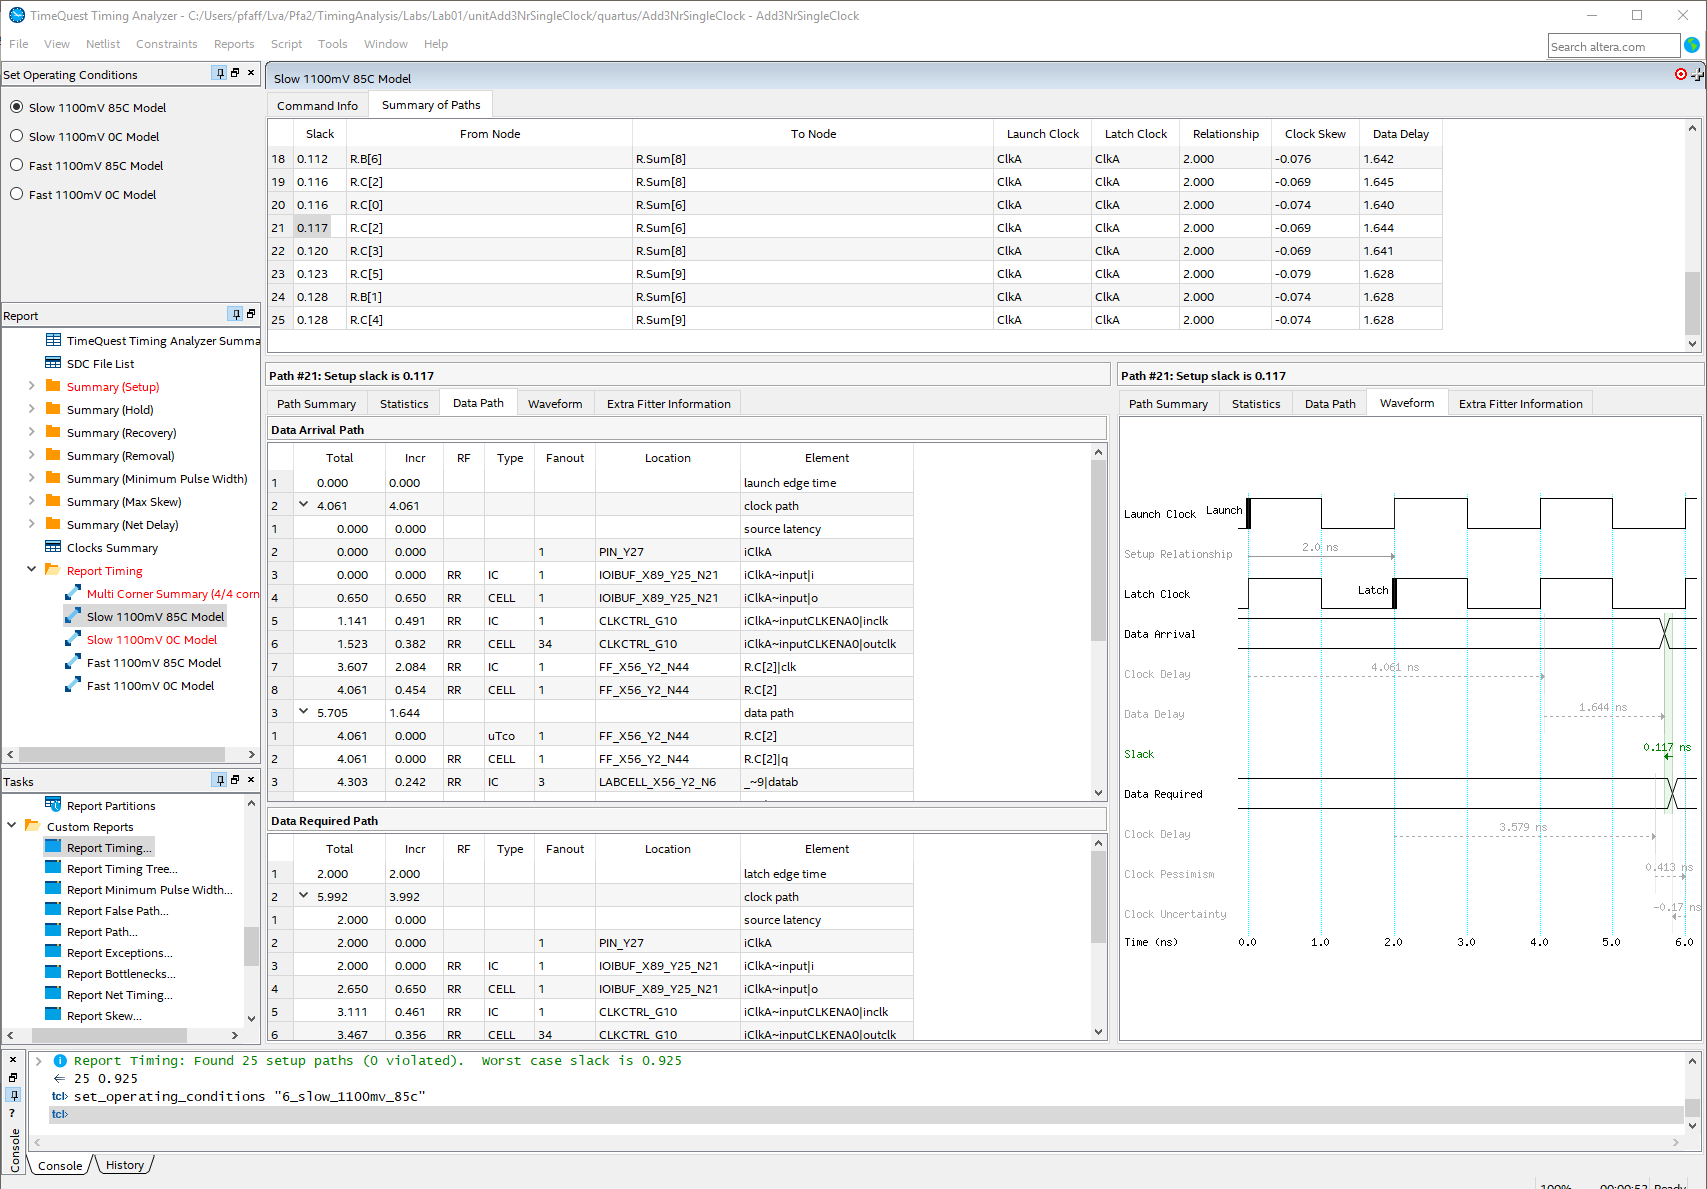
\includegraphics[width=\textwidth]{pic/TimeQuestReportTiming}
    \caption{\label{fig:ReportTiming}Results of \emph{Report Timing...}}
  \end{figure}

\end{aufgabe}

\begin{aufgabe}{Using two clocks}
  \begin{enumerate}
  \item Copy the complete project to some new directory and rename to
    Add3NrTwoClocks where needed.  You may simply delete the folders
    created by Quartus and open the qpf and qsf files in a text editor
    to do so.  Of course the VHDL files need adaption to.
  \item Enhance the VHDL description with a second clock port named
    \lstinline|iClkB|.
  \item The clock domain of ClkB should be separated clearly from the
    clock domain ClkA.  The registers residing in ClkB domain are the
    Sum registers.  Use separate records (reg set and constant for
    reset values) for clock domain ClkA and ClkB.  Also use separate
    processes to describe what is to be done in each domain.
  \item Later on we will add a PLL to generate the two clock signals,
    but for now we don't care on how they are generated.  They just
    come in from the outside in the form we will describe in our sdc
    file.
  \item Add a \verb|create_clock| command to the sdc file to describe
    clock ClkB.  Use the exactly same definition as for ClkA and
    analyse the timing of the design.  Note that the timing analyzer
    will take your clock definitions as absolute accurate.  This means
    both clock signals will have exactly the form you describe until
    eternity.  No phase shift, skew, flutter or whatever will happen
    to your clock signals now or in the future.

    Is the timing the same as in the example using a single clock if
    two identical clocks are used?
  \end{enumerate}
\end{aufgabe}

\end{document}


%%% Local Variables:
%%% mode: latex
%%% TeX-master: t
%%% End:
